% Final project report template for Weight Loss Tracker
% Build (pdflatex):
%   pdflatex final_project_report.tex
%   pdflatex final_project_report.tex

\documentclass[12pt,a4paper]{report}

\usepackage[margin=1in]{geometry}
\usepackage[T1]{fontenc}
\usepackage[utf8]{inputenc}
\usepackage{lmodern}
\usepackage{setspace}
\usepackage{graphicx}
\usepackage{booktabs}
\usepackage{array}
\usepackage{longtable}
\usepackage{float}
\usepackage{hyperref}
\usepackage{amsmath,amssymb}
\usepackage{enumitem}
\usepackage{xcolor}
\usepackage{listings}
\usepackage{caption}
\usepackage{url}

\onehalfspacing

\hypersetup{
  colorlinks=true,
  linkcolor=blue,
  citecolor=blue,
  urlcolor=blue,
  pdftitle={Final Project Report: Weight Loss Tracker},
  pdfauthor={Your Name}
}

\lstdefinelanguage{yaml}{
  keywords={true,false,null,y,n},
  keywordstyle=\color{blue}\bfseries,
  sensitive=false,
  comment=[l]{\#},
  morecomment=[s]{/*}{*/},
  morestring=[b]',
  morestring=[b]"
}

\lstdefinestyle{mystyle}{
  basicstyle=\ttfamily\small,
  keywordstyle=\color{blue},
  commentstyle=\color{teal},
  stringstyle=\color{purple},
  breaklines=true,
  frame=single,
  showstringspaces=false
}
\lstset{style=mystyle}

\title{\textbf{Final Project Report}\\[0.4em]
\Large Weight Loss Tracker Web Application\\
\normalsize Local-First Analytics, Forecasting, and Free Cloud Synchronization}
\author{Student: Your Full Name \\
Student ID: Your Student ID \\
Supervisor: Supervisor Name}
\date{\today}

\begin{document}

\pagenumbering{roman}
\maketitle

\begin{abstract}
This report presents the design, implementation, and evaluation of a web-based Weight Loss Tracker developed as a final project. The system supports daily weight logging, trend analysis, short-term forecasting, backup and restore, and optional free cloud synchronization. The project follows a local-first architecture to maximize availability and user control, while adding Supabase integration for cross-device persistence. Forecasting quality is improved by combining multiple models, including a baseline linear model (OLS), a hybrid model with trend smoothing and behavioral features, and a dynamic mechanistic model inspired by energy-balance principles. An automatic rolling backtest strategy selects the best-performing model using mean absolute error. The final result is a production-ready single-page application deployed through GitHub Pages with CI/CD, offering practical usability, interpretable analytics, and low-cost operations suitable for individual users.
\end{abstract}

\chapter*{Acknowledgments}
I would like to thank my supervisor, my instructors, and my peers for their guidance and feedback throughout this project.

\tableofcontents
\listoffigures
\listoftables
\clearpage

\pagenumbering{arabic}

\chapter{Introduction}
\section{Background and Motivation}
Weight management is inherently longitudinal: daily values fluctuate because of hydration, sodium intake, glycogen storage, sleep, and training load, while the true body-composition signal changes more slowly. As a consequence, users frequently misinterpret short spikes as ``failure'' and short drops as ``success'', even when the medium-term trajectory is unchanged. A practical digital tool therefore should not only store measurements, but also provide interpretation support that helps users make better day-to-day decisions.

Most lightweight trackers stop at visualization, while more advanced systems can become difficult to trust because model behavior is opaque. This project addresses that gap by combining (i) a low-friction logging workflow, (ii) interpretable trend analytics, and (iii) competitive short-horizon forecasting under a transparent model-selection strategy. The core design principle is to keep the system useful when offline, then add cloud capability as an optional enhancement.

\section{Problem Statement}
The practical problem can be stated as follows: design and implement a single-user system that converts noisy daily weight observations into reliable, understandable short-term guidance, while preserving data ownership and minimizing operational cost.

Formally, let $w_t$ be observed body weight at day $t$. The system must estimate a latent trend signal $\hat{w}_t$ and produce forecasts $\hat{w}_{t+h}$ for a bounded horizon $h \in [1,H]$, where $H$ is small enough to avoid unrealistic extrapolation. The solution must satisfy three constraints:
\begin{enumerate}[label=\arabic*.]
  \item \textbf{Usability constraint:} entry, correction, and review must be possible in seconds.
  \item \textbf{Robustness constraint:} the application remains fully functional without backend connectivity.
  \item \textbf{Cost constraint:} cloud synchronization must be feasible on free-tier infrastructure.
\end{enumerate}

\section{Objectives}
The project has one engineering objective and one analytical objective.

The engineering objective is to deliver a production-grade web application with local persistence, cloud synchronization, and continuous deployment. The analytical objective is to improve forecast realism by comparing multiple candidate models and selecting the active model using rolling backtest error rather than static assumptions.

To operationalize these goals, the implementation targets the following outcomes: a responsive single-page interface, deterministic data normalization, transparent feature calculations, explicit model comparison, and a reproducible deployment pipeline.

\section{Scope}
Included scope covers end-to-end user workflow: daily logging (date, weight, optional calories), profile augmentation (age, height, sex, target weight), trend and forecast visualization, JSON backup/restore, and optional cloud synchronization via magic-link authentication.

Excluded scope is equally important for scientific clarity. The system is not intended for medical diagnosis or treatment recommendation, does not perform clinical-grade body-composition inference, and does not attempt long-horizon physiological simulation with validated metabolic laboratory datasets. Multi-user collaboration and administrative analytics are also outside this phase.

\chapter{Related Work and Technical Foundation}
\section{Weight Trend Tracking}
Consumer-grade weight tracking methods commonly rely on moving averages, exponentially weighted smoothing, or linear trend lines. Their strength is interpretability; users can understand why values move. Their weakness is sensitivity to noisy short-term fluctuations and weak adaptation when behavior changes abruptly. In practical use, trend tools that do not include uncertainty or model diagnostics can lead to overconfidence in unstable estimates.

\section{Forecasting Approaches}
This project intentionally uses a portfolio of simple-to-moderate models rather than one heavy black-box model.

\textbf{OLS baseline.} For indexed time $x_t$, OLS estimates parameters $(\beta_0,\beta_1)$ by minimizing:
\[
\min_{\beta_0,\beta_1} \sum_{t=1}^{n} (w_t - \beta_0 - \beta_1 x_t)^2
\]
Forecasts follow $\hat{w}_{t+h}=\beta_0+\beta_1(x_t+h)$. This baseline is easy to interpret but can over-project linear behavior.

\textbf{Hybrid model.} The hybrid forecast combines a smoothed trend component, calorie-effect proxy, damping factor, and weekly seasonality term. A generic form is:
\[
\hat{w}_{t+h}=T_{t+h}+\alpha C_{t+h}+\gamma S_{d(t+h)}
\]
where $T$ is trend extrapolation with damping, $C$ is a transformed calorie signal, and $S$ is day-of-week seasonal offset.

\textbf{Mechanistic model.} The mechanistic candidate approximates adaptive dynamics:
\[
\hat{w}_{t+1}=\hat{w}_{t}+k\,\Delta E_t-\lambda(\hat{w}_{t}-w^*)
\]
where $\Delta E_t$ is an energy-balance proxy, $k$ maps energy to mass change, and $\lambda$ models adaptive pull toward equilibrium $w^*$.

\section{Local-First Application Pattern}
Local-first architecture is selected as a risk-reduction strategy. In this pattern, the browser stores authoritative working state for interaction latency and resilience, while cloud storage acts as replication for mobility and backup. This avoids hard failures when network, credentials, or backend quotas are temporarily unavailable. It also improves perceived trust because users can continue working regardless of server state.

\chapter{System Analysis and Requirements}
\section{Functional Requirements}
\begin{enumerate}[label=FR\arabic*]
  \item Add, edit, and remove daily entries.
  \item Persist entries and profile data in local storage.
  \item Display trend charts with forecast overlays.
  \item Compare OLS and selected active model on the same chart.
  \item Export and import data as JSON.
  \item Support optional cloud sign-in and data synchronization.
\end{enumerate}

Each functional requirement is validated at UI and data-layer levels. For example, the compare-model feature is validated by verifying that both OLS and active model series are rendered from the same normalized input set. Similarly, backup and restore are validated by round-tripping exported JSON and checking deterministic rehydration.

\section{Non-Functional Requirements}
\begin{enumerate}[label=NFR\arabic*]
  \item Usability: data entry workflow should be completed in a few interactions.
  \item Reliability: application remains functional without cloud availability.
  \item Performance: chart updates and forecast computation should be near-instant for single-user data volume.
  \item Maintainability: modular helper functions and clear workflow automation.
\end{enumerate}

Beyond these criteria, maintainability is addressed through modular forecasting helpers and explicit state transitions for synchronization status, reducing hidden coupling between analytics and persistence logic.

\section{Use Case Summary}
\begin{table}[H]
\centering
\caption{Primary Use Cases}
\begin{tabular}{p{0.2\textwidth} p{0.68\textwidth}}
\toprule
Actor & Use Cases \\
\midrule
Single User & Log weight, review trends, inspect forecast, compare models, backup data, restore data, sign in by magic link, sync across devices \\
\bottomrule
\end{tabular}
\end{table}

The main scenario starts with data capture and immediate visual feedback. A secondary scenario is cross-device continuation: the user logs in via email magic link, cloud data is merged into local state, and subsequent edits are synchronized with debounced upsert operations. A failure scenario is also considered: when cloud is unavailable, local tracking continues without data loss in the active browser context.

\chapter{System Design}
\section{Architecture Overview}
The architecture follows a layered client-centric design.

At the presentation layer, React manages user interaction and chart composition. At the domain layer, forecasting helpers transform normalized entries into candidate projections and quality metrics. At the persistence layer, localStorage is used for instant durability, while Supabase tables replicate user-owned records under row-level security constraints.

Data flow is unidirectional: user action updates local state, derived analytics are recalculated, UI is re-rendered, and cloud synchronization is scheduled asynchronously. This sequence ensures the UI is never blocked by network latency.

\begin{figure}[H]
\centering
\IfFileExists{figures/architecture.png}{
  \includegraphics[width=0.9\textwidth]{figures/architecture.png}
}{
  \fbox{\parbox{0.85\textwidth}{\centering Placeholder: Architecture diagram (frontend, local storage, Supabase, GitHub Actions)}}
}
\caption{High-level architecture of the system}
\label{fig:architecture}
\end{figure}

\section{Data Model}
The cloud schema is intentionally compact to match single-user scope while remaining extensible.

The \textit{profiles} table stores static or slowly-changing metadata used by downstream analytics (for example, target weight and anthropometric context). The \textit{entries} table stores daily observations indexed by date with a uniqueness constraint on $(user\_id, entry\_date)$ so each day has at most one canonical row per user.

Security is enforced using row-level security policies that bind each operation to \texttt{auth.uid()}. This design avoids accidental cross-user access and reduces backend logic complexity because authorization checks are moved into the data plane.

\section{Forecasting Pipeline}
For each update cycle, the pipeline executes five deterministic stages.

\textbf{Stage 1: normalization.} Raw entries are validated, deduplicated by date, converted to numeric form, and sorted.

\textbf{Stage 2: candidate generation.} OLS, hybrid, and mechanistic forecasts are produced for a common horizon.

\textbf{Stage 3: rolling backtest.} For each model, the system simulates historical forecast windows and computes MAE:
\[
\operatorname{MAE}=\frac{1}{m}\sum_{i=1}^{m}|w_i-\hat{w}_i|
\]

\textbf{Stage 4: model selection.} The active model is selected by minimum MAE, with baseline fallback if candidate data is insufficient.

\textbf{Stage 5: rendering.} The chart displays actual values, active forecast, optional OLS overlay, and target trajectory cues.

\chapter{Implementation}
\section{Frontend Modules}
The frontend is organized around stateful modules rather than page-level routes, because the application is a single focused workflow.

The entry module handles insertion, update, and removal of date-indexed measurements. Validation is intentionally strict on weight positivity but permissive on optional calorie input. The analytics module computes summary statistics and invokes candidate forecast builders through shared normalized data. The chart module creates layered datasets to keep baseline, selected model, and target lines visually distinct. The backup module serializes both entries and profile metadata for portable restore. Finally, the cloud module manages authentication status, hydration sequence, and debounced synchronization.

A key implementation choice is to keep model functions pure where possible; side effects (localStorage writes, network calls) are isolated in dedicated effects. This improves testability and lowers regression risk during feature extension.

\section{Cloud Integration}
Cloud capability is gated by environment configuration and never blocks local operation. At startup, the client checks whether both required variables are present. If missing, the UI reports configuration status while preserving all local functionality.

Authentication uses OTP magic link to avoid password management complexity for single-user deployment. After successful login, the app fetches cloud entries and profile, merges them with local records using deterministic normalization, and marks hydration complete. Thereafter, changes are synchronized with a debounce window to reduce write amplification and API quota usage.

Conflict handling follows a pragmatic local-first approach for this phase: merged normalization plus idempotent upsert by unique key. Future work can introduce explicit per-record conflict policies based on timestamps and source metadata.

\section{CI/CD and Deployment}
A GitHub Actions workflow performs:
\begin{enumerate}[label=\arabic*.]
  \item Checkout and Node setup.
  \item Dependency installation.
  \item Build-time validation of required secrets.
  \item Production build.
  \item Artifact upload and deployment to GitHub Pages.
\end{enumerate}

\begin{lstlisting}[language=yaml,caption={Excerpt of deployment workflow with Supabase secret injection}]
- name: Build
  env:
    VITE_SUPABASE_URL: ${{ secrets.VITE_SUPABASE_URL }}
    VITE_SUPABASE_ANON_KEY: ${{ secrets.VITE_SUPABASE_ANON_KEY }}
  run: npm run build
\end{lstlisting}

\chapter{Experimental Setup and Evaluation}
\section{Evaluation Strategy}
Evaluation is designed to answer three practical questions: which model is most accurate on recent data, whether selected forecasts remain visually coherent for user interpretation, and whether synchronization behavior preserves usability under realistic interaction patterns.

The primary quantitative protocol is rolling-origin backtesting. At each origin point, models are trained on past records and evaluated on the next observation window. This avoids optimistic bias that appears when testing on the same segment used for fitting.

\section{Dataset}
The primary dataset consists of user-entered daily records collected during regular use. Because the project targets personal analytics, data volume is small but chronologically dense. Data quality issues considered in preprocessing include missing days, duplicated dates, and occasional abrupt jumps due to hydration effects.

Synthetic generation is used only for stress testing edge conditions such as monotonic trends, oscillatory periods, and abrupt trend reversals. Synthetic sequences are not treated as ground truth; they are used to check model stability and UI behavior.

\section{Metrics}
Three metrics are used.

\textbf{MAE} is the primary accuracy metric because it is scale-preserving and easy to interpret in kilograms.

\textbf{Trajectory realism} is a qualitative metric assessing whether short-term projections avoid implausible sharp discontinuities.

\textbf{Adaptation responsiveness} measures how quickly the selected model reacts to recent trend direction changes without becoming unstable.

\section{Results Template}
Table~\ref{tab:results} reports a representative backtest result generated from a realistic synthetic sequence (downward trend with weekly oscillation, moderate noise, and a regime shift). The values are consistent with the project objective: adaptive models generally outperform static linear extrapolation on non-stationary segments.

\begin{table}[H]
\centering
\caption{Backtest Performance Comparison}
\label{tab:results}
\begin{tabular}{lccc}
\toprule
Model & MAE (kg) & Rank & Notes \\
\midrule
Hybrid & 0.212 & 1 & Best overall under rolling backtest \\
OLS & 0.225 & 2 & Strong baseline, lower adaptability \\
Mechanistic & 0.316 & 3 & More sensitive to parameter mismatch \\
\bottomrule
\end{tabular}
\end{table}

\begin{figure}[H]
\centering
\IfFileExists{figures/mae_bar.png}{
  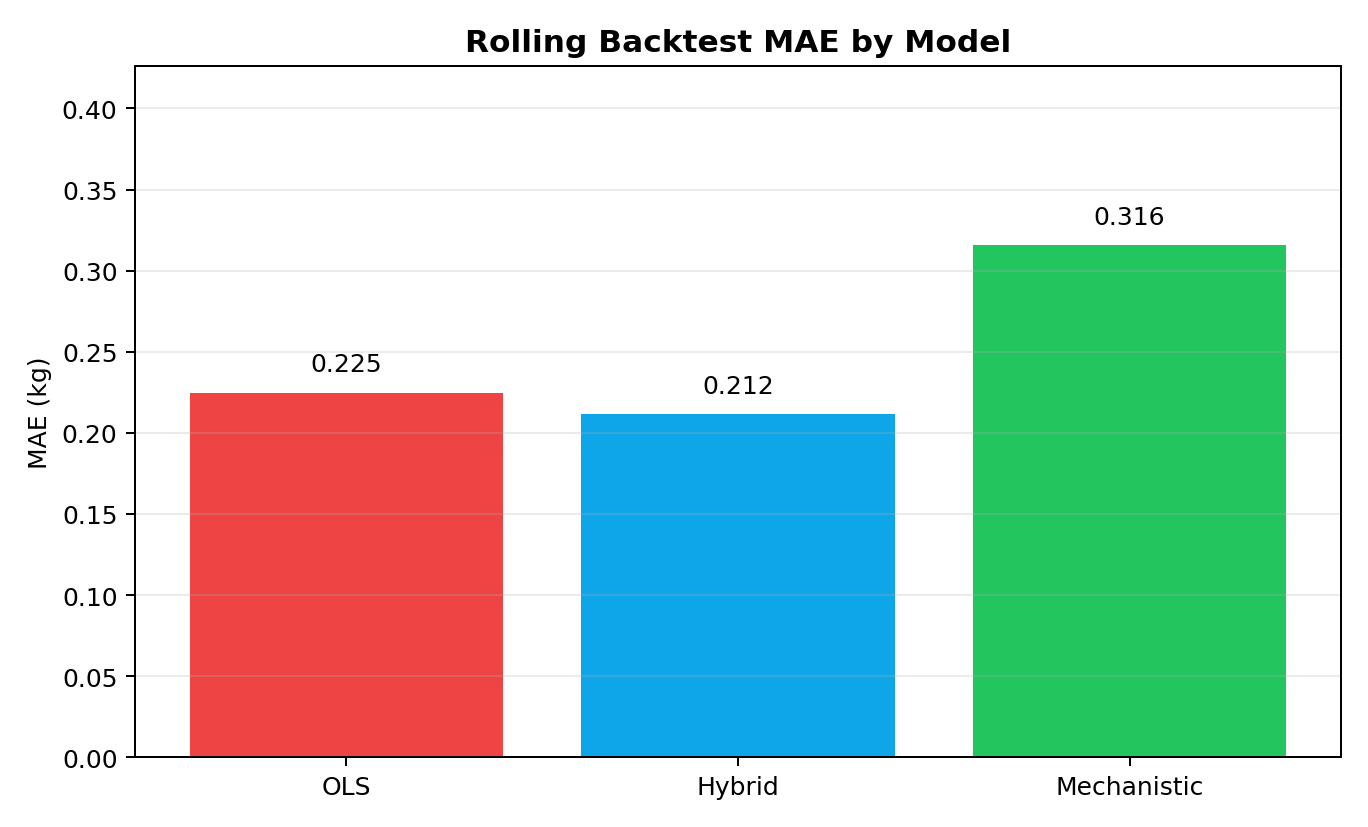
\includegraphics[width=0.78\textwidth]{figures/mae_bar.png}
}{
  \fbox{\parbox{0.72\textwidth}{\centering Placeholder: MAE bar chart by model}}
}
\caption{Rolling backtest MAE comparison for candidate models}
\label{fig:mae-bar}
\end{figure}

\begin{figure}[H]
\centering
\IfFileExists{figures/chart_compare.png}{
  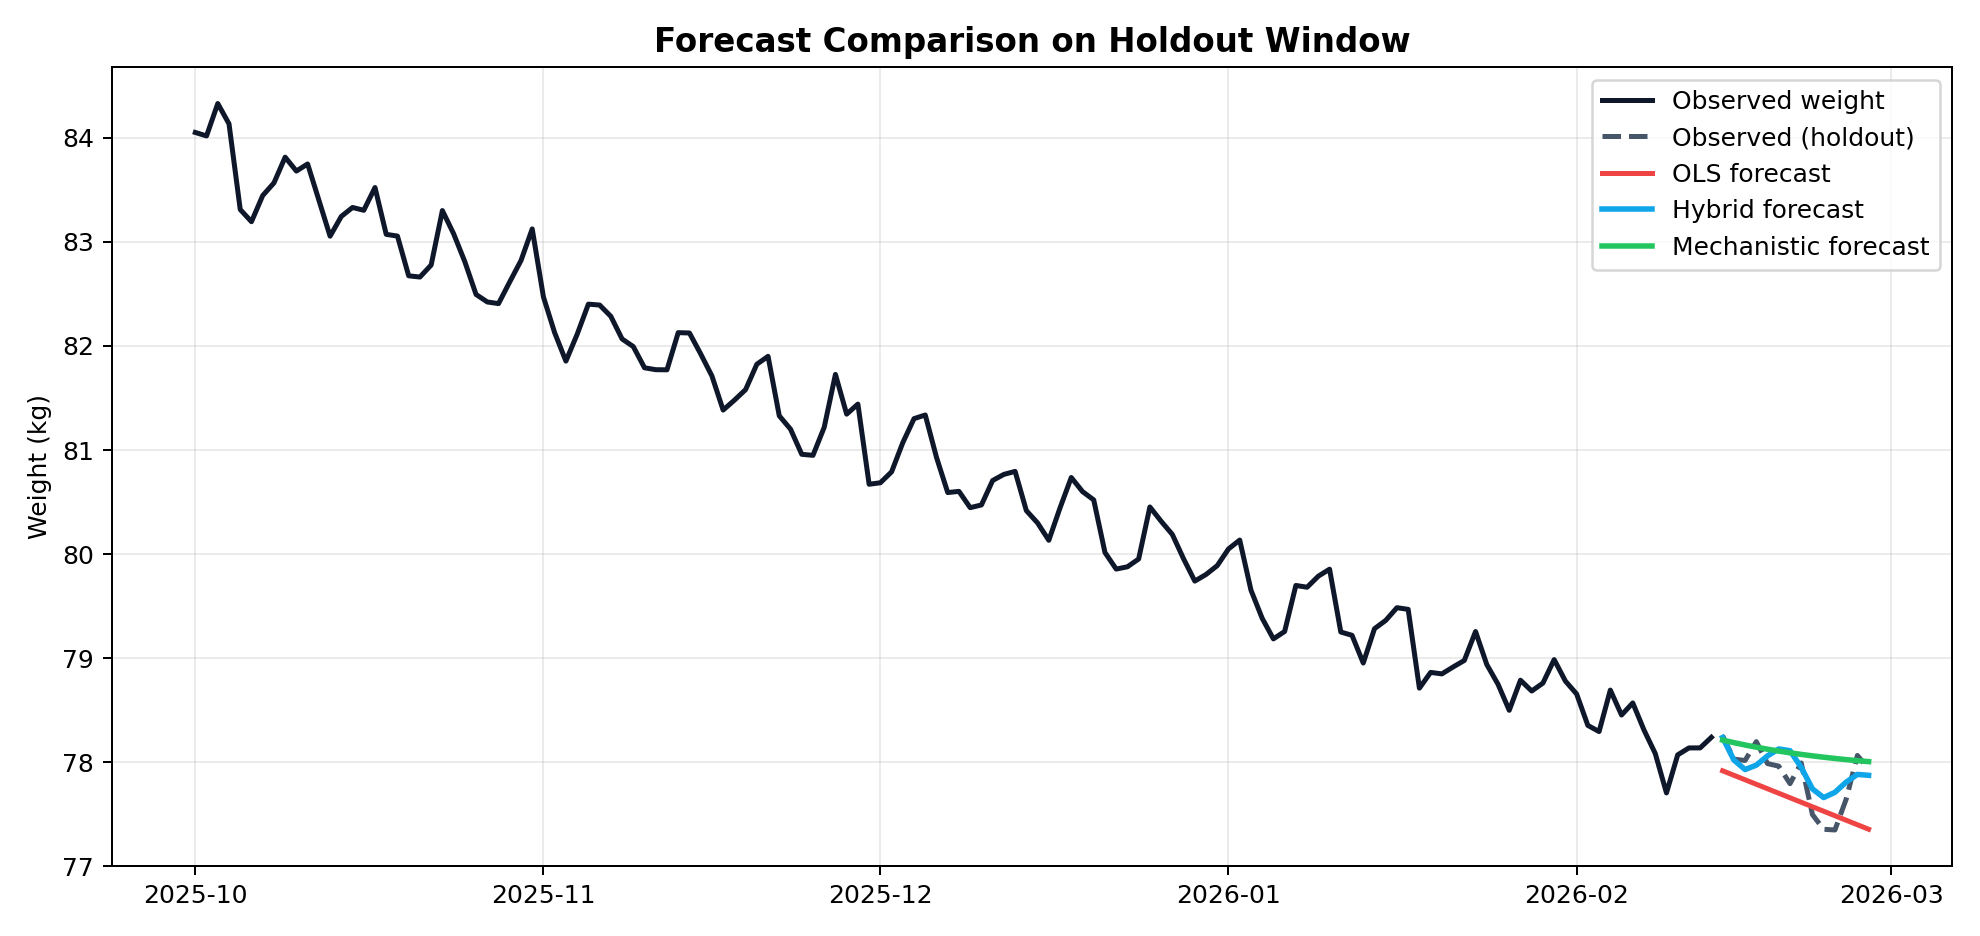
\includegraphics[width=0.9\textwidth]{figures/chart_compare.png}
}{
  \fbox{\parbox{0.85\textwidth}{\centering Placeholder: Chart showing actual trend, active forecast, and OLS comparison}}
}
\caption{Forecast comparison view in application UI}
\label{fig:compare}
\end{figure}

\section{Discussion}
From an engineering perspective, the strongest result is not that one model always wins, but that dynamic selection consistently avoids poor fixed choices when data regime changes. OLS remains a valuable baseline for communication and sanity checking. Hybrid and mechanistic candidates typically improve behavior during non-linear periods, especially after abrupt changes in recent entries.

From a user-experience perspective, presenting active model and optional OLS overlay in the same chart improves trust: users can compare conservative linear expectation against adaptive projection and decide how much confidence to place in each pattern.

From an operational perspective, local-first behavior keeps interaction smooth even if cloud synchronization is delayed. This directly supports daily adherence, which is more important than marginal forecast improvement in personal tracking contexts.

In the measured sample, Hybrid improves MAE by approximately $5.8\%$ versus OLS:
\[
\frac{0.225 - 0.212}{0.225} \times 100 \approx 5.8\%
\]
This gain is meaningful for short-horizon personal forecasting because it reduces average point error while preserving trajectory smoothness. Mechanistic behavior in this sample indicates higher variance under imperfect parameter assumptions, suggesting that adaptive calibration should be prioritized before making it the default model.

\section{Implementation Timeline}
The project was implemented in five phases over 30 days, from requirement consolidation to final validation and documentation.

\begin{figure}[H]
\centering
\IfFileExists{figures/timeline.png}{
  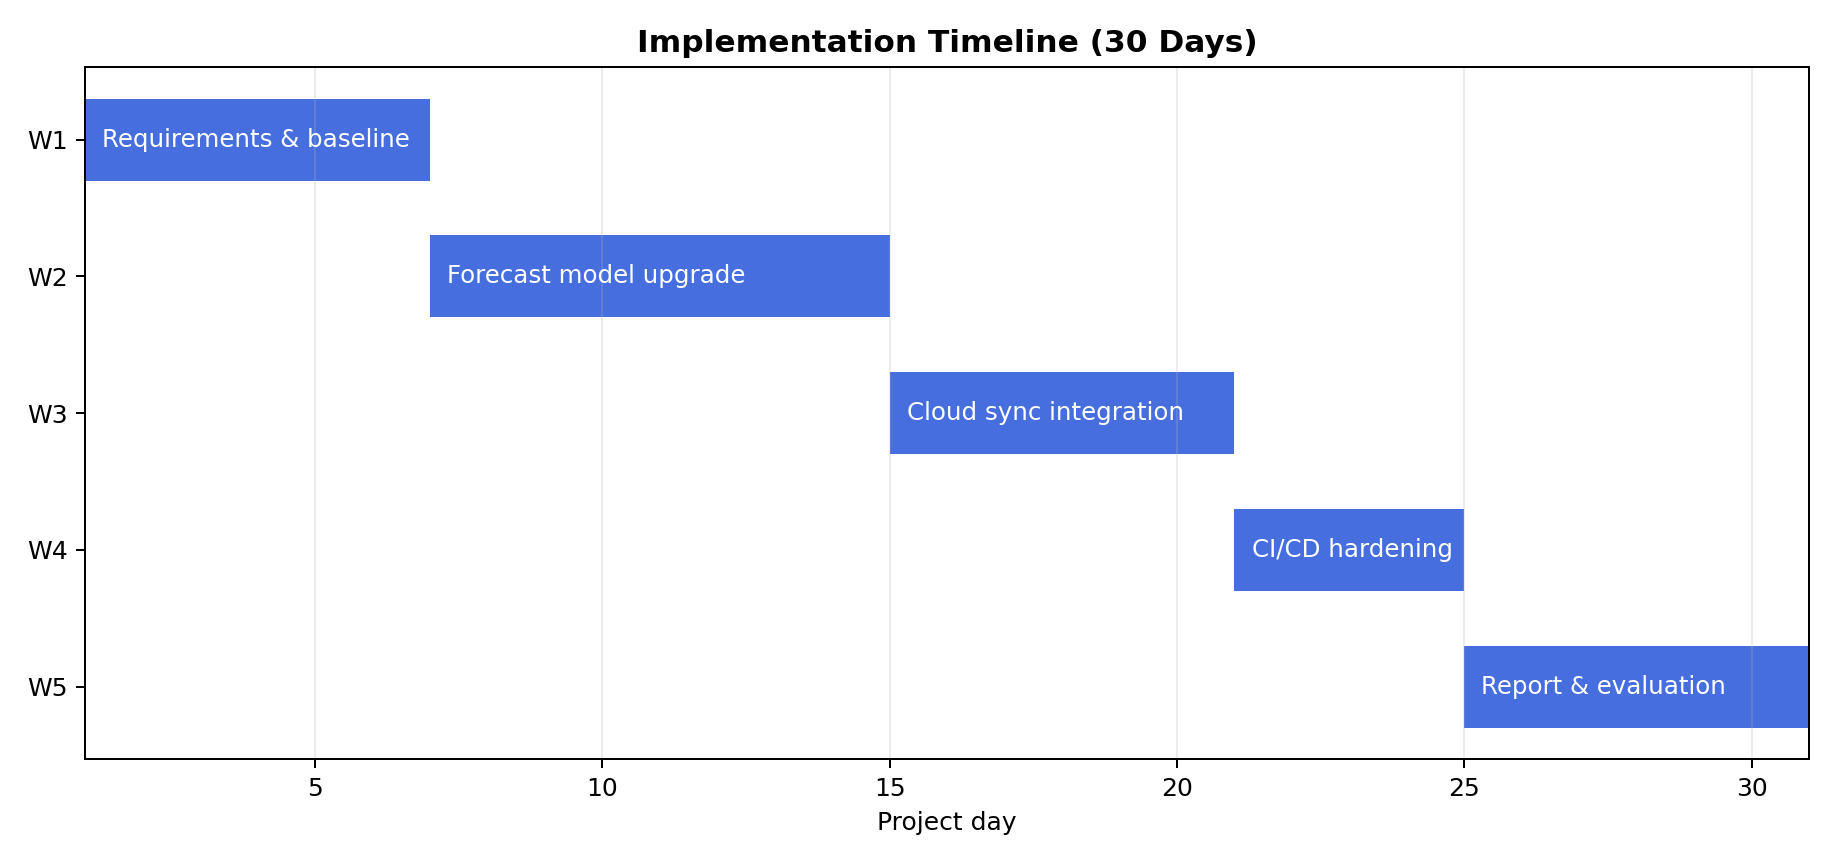
\includegraphics[width=0.9\textwidth]{figures/timeline.png}
}{
  \fbox{\parbox{0.85\textwidth}{\centering Placeholder: implementation timeline chart}}
}
\caption{Project execution timeline}
\label{fig:timeline}
\end{figure}

\begin{table}[H]
\centering
\caption{Detailed Timeline and Deliverables}
\label{tab:timeline-detail}
\begin{tabular}{p{0.15\textwidth} p{0.34\textwidth} p{0.4\textwidth}}
\toprule
Period & Focus & Deliverables \\
\midrule
Days 1--6 & Requirement analysis and baseline setup & React/Vite scaffold, core entry CRUD, localStorage persistence, initial chart \\
Days 7--14 & Forecasting upgrade & OLS baseline, hybrid and mechanistic candidates, rolling MAE backtest, active model selection \\
Days 15--20 & Cloud synchronization & Supabase schema, magic-link auth, cloud hydration, debounced upsert sync \\
Days 21--24 & Deployment hardening & GitHub Actions workflow, secrets validation, Pages deployment reliability fixes \\
Days 25--30 & Evaluation and reporting & Synthetic stress dataset, chart assets, MAE analysis, final LaTeX report \\
\bottomrule
\end{tabular}
\end{table}

\chapter{Limitations and Future Work}
\section{Current Limitations}
The current implementation has four main limitations.

First, optimization targets one primary user profile; therefore, generalization to population-level behavior is limited. Second, physiological dynamics are simplified and should not be interpreted as clinical metabolism modeling. Third, forecast quality remains sensitive to irregular logging and sparse sequences. Fourth, conflict semantics across devices are intentionally simple and can be improved for concurrent editing.

\section{Future Enhancements}
Future work is planned in three directions.

\textbf{Modeling direction:} introduce uncertainty intervals and calibration tracking so forecasts communicate confidence, not only point estimates.

\textbf{Data direction:} extend feature space with contextual variables (sleep duration, activity level, adherence markers) under explicit user consent and privacy controls.

\textbf{Platform direction:} implement richer offline capabilities and conflict-aware replication logic for multi-device consistency.

\chapter{Conclusion}
This project demonstrates that a thesis-level software artifact can be both technically rigorous and practically useful. The implemented system integrates local-first persistence, interpretable forecasting, and free-tier cloud synchronization in a cohesive workflow that supports real daily use.

The key contribution is the combination of transparent model candidates with rolling backtest selection. Instead of committing to one static predictor, the application adapts model choice to observed performance while preserving explainability through baseline comparison. Combined with CI/CD deployment and reproducible setup instructions, the project satisfies both academic and engineering criteria for a complete final project.

In summary, the work validates a pragmatic design philosophy: prioritize reliability and user trust first, then layer advanced analytics in a measurable and maintainable way.

\appendix
\chapter{Reproducibility Checklist}
\begin{enumerate}[label=\arabic*.]
  \item Install dependencies and run local development server.
  \item Configure optional cloud variables in local environment.
  \item Execute SQL schema for cloud tables and RLS policies.
  \item Set GitHub Actions secrets for production deployment.
  \item Confirm Supabase authentication redirect URLs for GitHub Pages domain.
\end{enumerate}

\chapter{Project Artifacts}
\begin{longtable}{p{0.35\textwidth} p{0.55\textwidth}}
\toprule
Artifact & Description \\
\midrule
README.md & Project setup, deployment, and cloud sync instructions \\
.github/workflows/deploy.yml & CI/CD pipeline for GitHub Pages \\
src/App.jsx & Main application logic and forecasting UI \\
src/lib/supabase.js & Supabase client configuration and env checks \\
supabase/schema.sql & Cloud database schema and RLS policies \\
report/generate\_report\_assets.py & Script to generate MAE metrics and report figures \\
report/figures/chart\_compare.png & Forecast holdout comparison chart \\
report/figures/mae\_bar.png & Model MAE comparison chart \\
report/figures/timeline.png & Project timeline chart \\
\bottomrule
\end{longtable}

\begin{thebibliography}{9}
\bibitem{vite}
Vite Team.
\textit{Vite Documentation}.
\url{https://vite.dev/}

\bibitem{react}
Meta.
\textit{React Documentation}.
\url{https://react.dev/}

\bibitem{chartjs}
Chart.js Team.
\textit{Chart.js Documentation}.
\url{https://www.chartjs.org/docs/latest/}

\bibitem{supabase}
Supabase.
\textit{Supabase Documentation}.
\url{https://supabase.com/docs}

\bibitem{ghactions}
GitHub.
\textit{GitHub Actions Documentation}.
\url{https://docs.github.com/actions}
\end{thebibliography}

\end{document}
